\section{Presentation of experimental or analytical results/descriptions of final constructed product}
在这一节我们主要讨论模型的测试结果和模型进一步改进的空间。


\subsection{带入测试集验证准确度}

在这里我们将训练好的模型应用到额外准备好的测试集上,计算模型的准确度。

\autoref{tab:model_accuracy}是模型在测试集上的准确度:(准确度定义为标签与模型预测一致的样本数占总样本数的比例)

\begin{figure}[htbp]
    \centering
    \begin{minipage}{0.45\textwidth}
        \centering
        \captionof{table}{Model accuracy on test set}
        \begin{tabular}{cc}
            \toprule
            Category & Accuracy(\%) \\
            \midrule
            Normal & 98.4 \\
            Horizontal Line & 95.6 \\
            Vertical Line & 80.0 \\
            Slope & 96.1 \\
            Other & 95.2 \\
            \bottomrule
        \end{tabular}
        \label{tab:model_accuracy}
    \end{minipage}
    \begin{minipage}{0.45\textwidth}
        \centering
        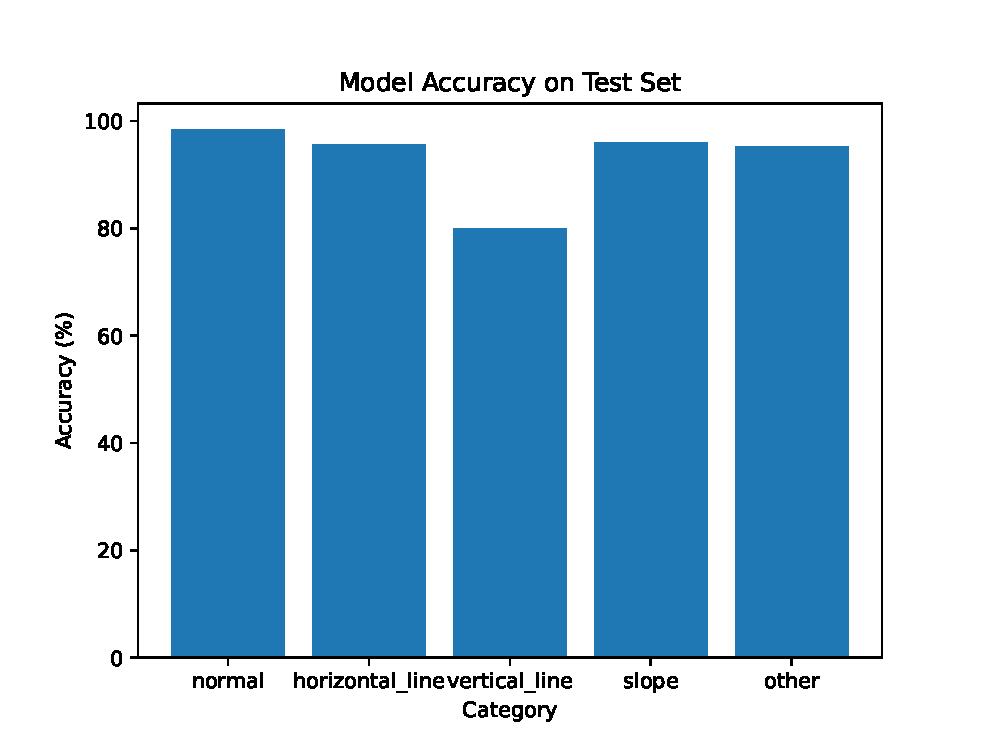
\includegraphics[width=\textwidth]{./fig/assistplot/accuracy.eps}
        \captionof{figure}{Model Accuracy on Test Set}
        \label{fig:accuracy_histogram}
    \end{minipage}
\end{figure}


可见,模型预测结果在normal上表现较好,而在vertical\_line上表现较差。这可能是由于用于测试的样本量较少,导致模型学习不足,难以判断。


\subsection{模型的进一步提高(改变输入分辨率)}

在这里我们讨论模型的进一步提高的空间。

将高分辨率图片缩放为InceptionV3模型默认的299x299大小的确可能导致信息和细节的丢失,特别是对于原始分辨率远高于此标准的图像。例如,从VHX7000设备采集的2880x2160分辨率图像就含有大量的细节,直接缩放可能不利于模型捕捉到所有的细微差别,尤其是在医学影像或其他细节丰富的领域。

改变模型的输入层接受更大的图片尺寸是一个潜在的解决方案。这样做的优势是它允许模型处理更高分辨率的图像,保留更多的原始信息和细节,可能导致更好的性能和更高的准确度。此外InceptionV3的架构设计有助于处理更大图片,因为其含有多个大小不一的卷积核,这使得它能够捕捉不同尺度的特征。

受制于实验室机器性能(显存为16G),在这里将图像缩放到分别为原图像的0.4倍,即1152*864,进行再一次训练。

新的模型为model4,训练效果如下所示:

\begin{figure}[H]
    \centering
    \begin{minipage}{0.45\textwidth}
        \centering
        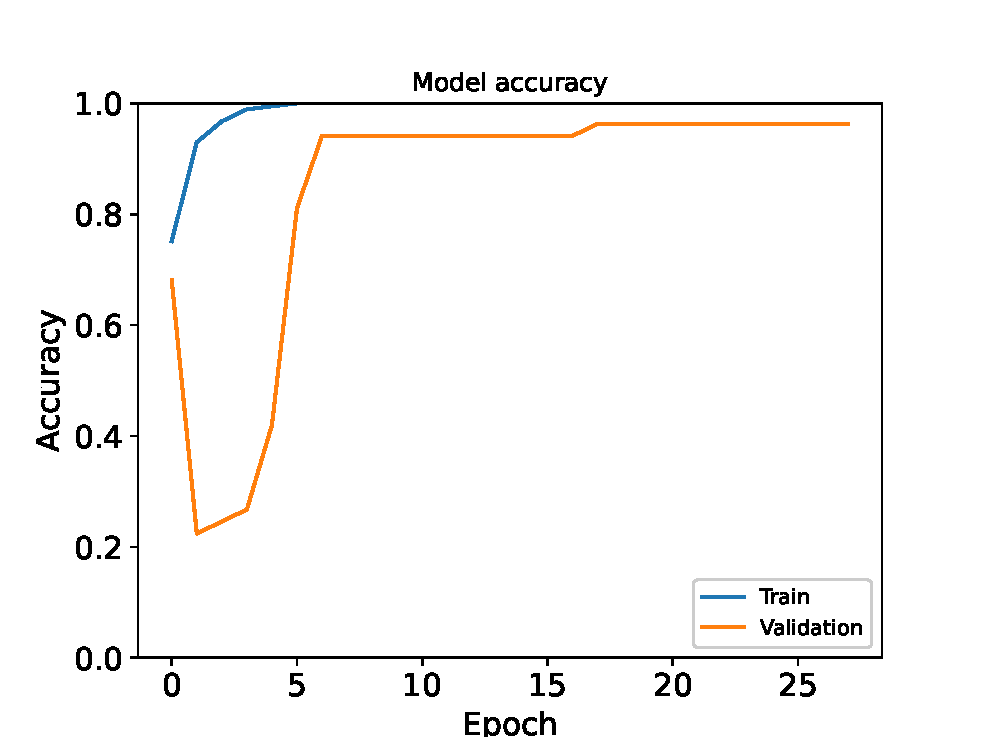
\includegraphics[width=\textwidth]{./fig/model4/accuracy4.eps}
        \caption{Model-4 accuracy}
        \label{fig:model4_accuracy}
    \end{minipage}
    \begin{minipage}{0.45\textwidth}
        \centering
        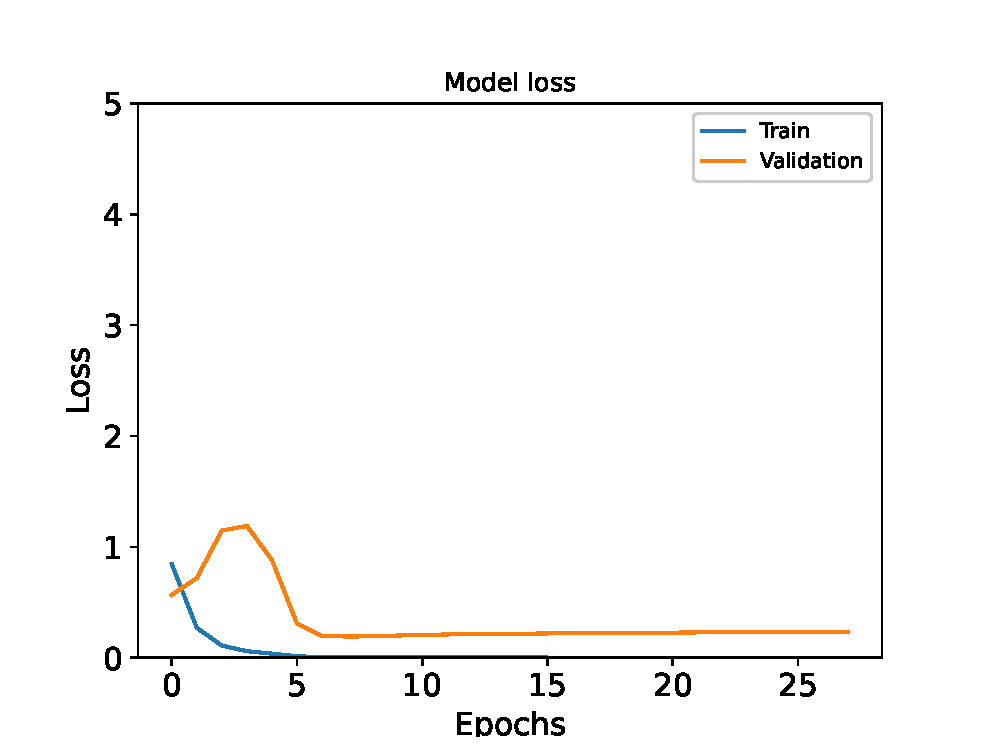
\includegraphics[width=\textwidth]{./fig/model4/loss4.eps}
        \caption{Model-4 loss}
        \label{fig:model4_loss}
    \end{minipage}
\end{figure}

观察训练准确度和损失随步长的变化可以发现,模型的性能有惊人的明显提升。训练和验证准确度都接近1,同时验证损失降至15\%左右,这通常表明模型具有很强的泛化能力。这种情况下,模型不仅在训练数据上表现出色,而且能够很好地泛化到新的、未见过的数据上。

将其再一次带入测试集进行准确度评估,结果如\autoref{tab:model_accuracy2}:

\begin{table}
    \centering
    \caption{model accuracy on test set}
    \begin{tabular}{cccccc}
        \toprule
        & normal & horizental\_line & vertical\_line & slope & other \\
        \midrule
        accuracy(\%) & 98.4 & 96.7 & 85.6 & 96.5 & 96.5 \\
        \bottomrule
    \end{tabular}
    \label{tab:model_accuracy2}
    \end{table}

对比修改分辨率前后的模型准确度,可以发现模型的准确度虽有提升但并不显著的,可能是由于准确度已经很接近于1,提升的空间较小导致的。


\subsection{探究机器的最佳切削角}

使用预先准备好的各个切削角度的图片,从8-12度,每0.5度一个样本,一共9组数据,每组数据包含100张图片,使用模型4来评估每组的良品率。此时,找到良品率最高的数据组,即为该机器的最佳切削角度。

\begin{figure}[htbp]
    \centering
    \begin{minipage}{0.4\textwidth}
        \centering
        \captionof{table}{Normal accuracy on different angle}
        \begin{tabular}{cc}
            \toprule
            Angle & Accuracy(\%) \\
            \midrule
            8 & 80 \\
            8.5 & 81.5 \\
            9 & 83.5 \\
            9.5 & 93.3 \\
            10 & 96.6 \\
            10.5 & 88.8 \\
            11 & 84.2 \\
            11.5 & 66.6 \\
            12 & 62.2 \\
            \bottomrule
        \end{tabular}
        \label{tab:model_accuracy_angle}
    \end{minipage}
    \begin{minipage}{0.55\textwidth}
        \centering
        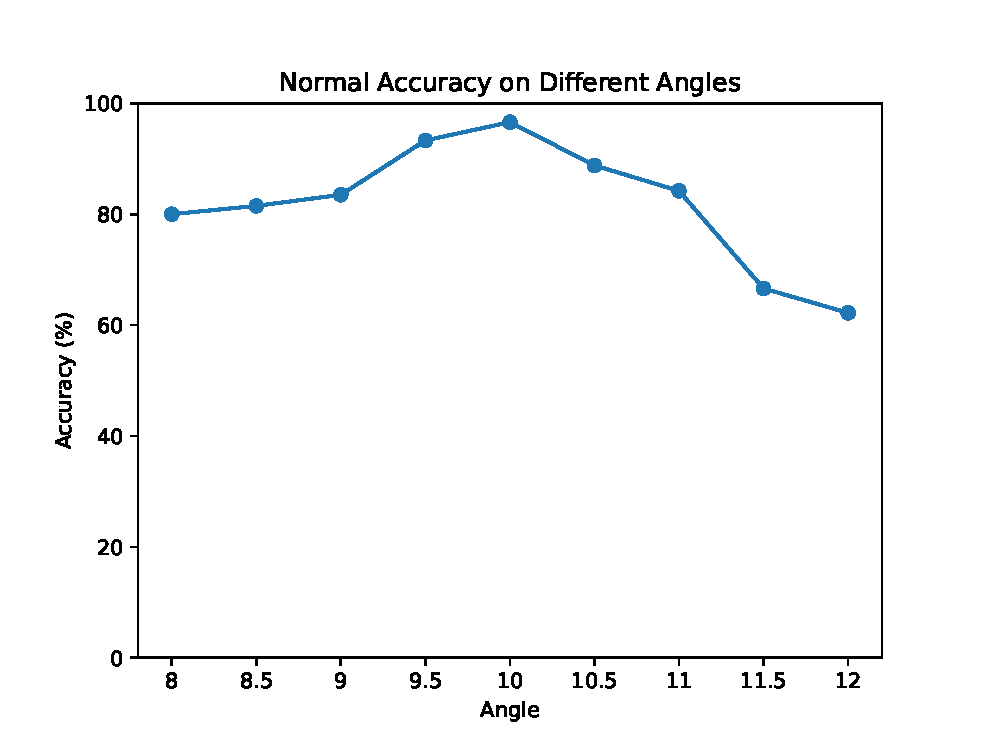
\includegraphics[width=\textwidth]{./fig/assistplot/angle_accuracy.eps}
        \captionof{figure}{Model Accuracy on Different Angle}
        \label{fig:angle_accuracy_histogram}
    \end{minipage}
\end{figure}

由\autoref{tab:model_accuracy_angle}可知,最佳切削角度为10度。

另外,从\autoref{fig:angle_accuracy_histogram}得出若要在保证切削质量为百分之80的情况下,切削角度应在9度到10.5度之间。


\subsection{模型通用性}

在上文的实验中我们采用的是鱼的卵巢为组织切片,而在实际应用中,我们可能会遇到其他组织切片,如其他器官或其他动物标本等。因此,我们需要考虑模型的通用性。

在这里有另一组已经采集好的数据集,是鱼的肺切片,在这一共将其分成4类,分别是good, normal, bad,other 四类(样本如\autoref{fig:good_fish_lung}到\autoref{fig:other_fish_lung})。现在更改输入数据集,保持原有model4架构不变,采用1152*864分辨率图片作为输入数据进行训练。

\begin{figure}[H]
    \centering
    \begin{minipage}{0.45\textwidth}
        \centering
        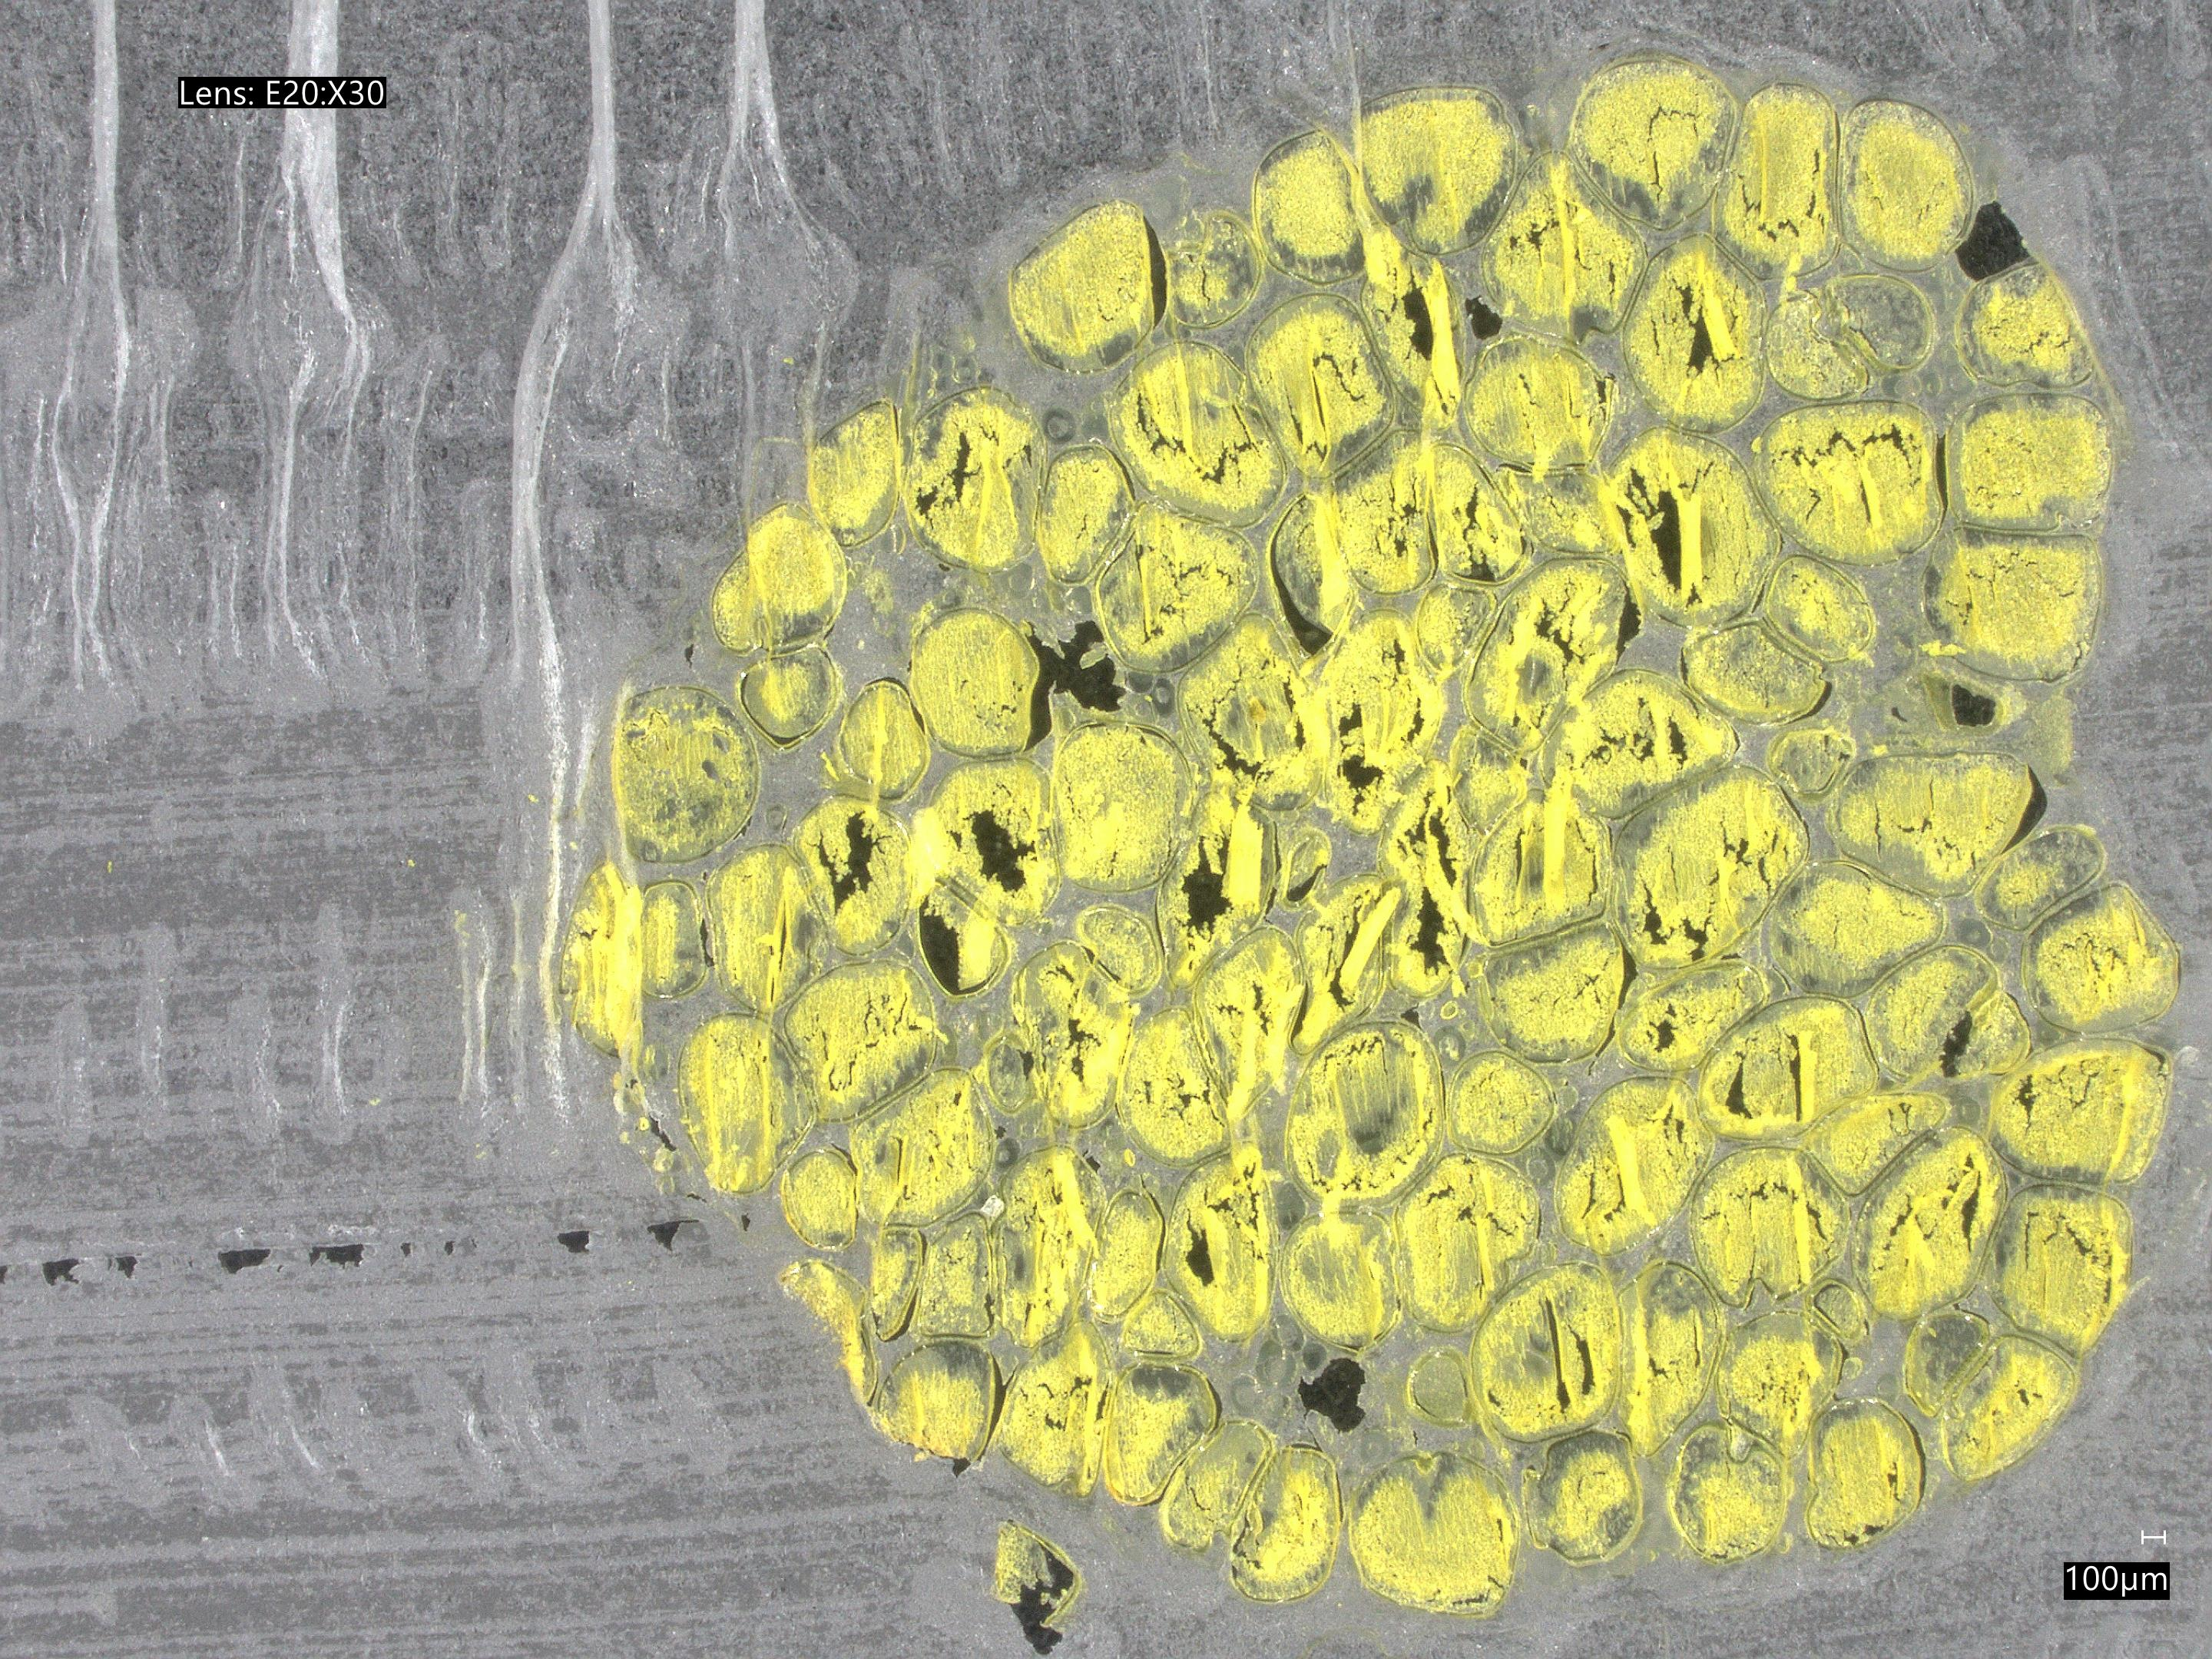
\includegraphics[width=\textwidth]{./fig/fish_lung/good20240313_144138.jpg}
        \caption{good fish lung}
        \label{fig:good_fish_lung}
    \end{minipage}
    \begin{minipage}{0.45\textwidth}
        \centering
        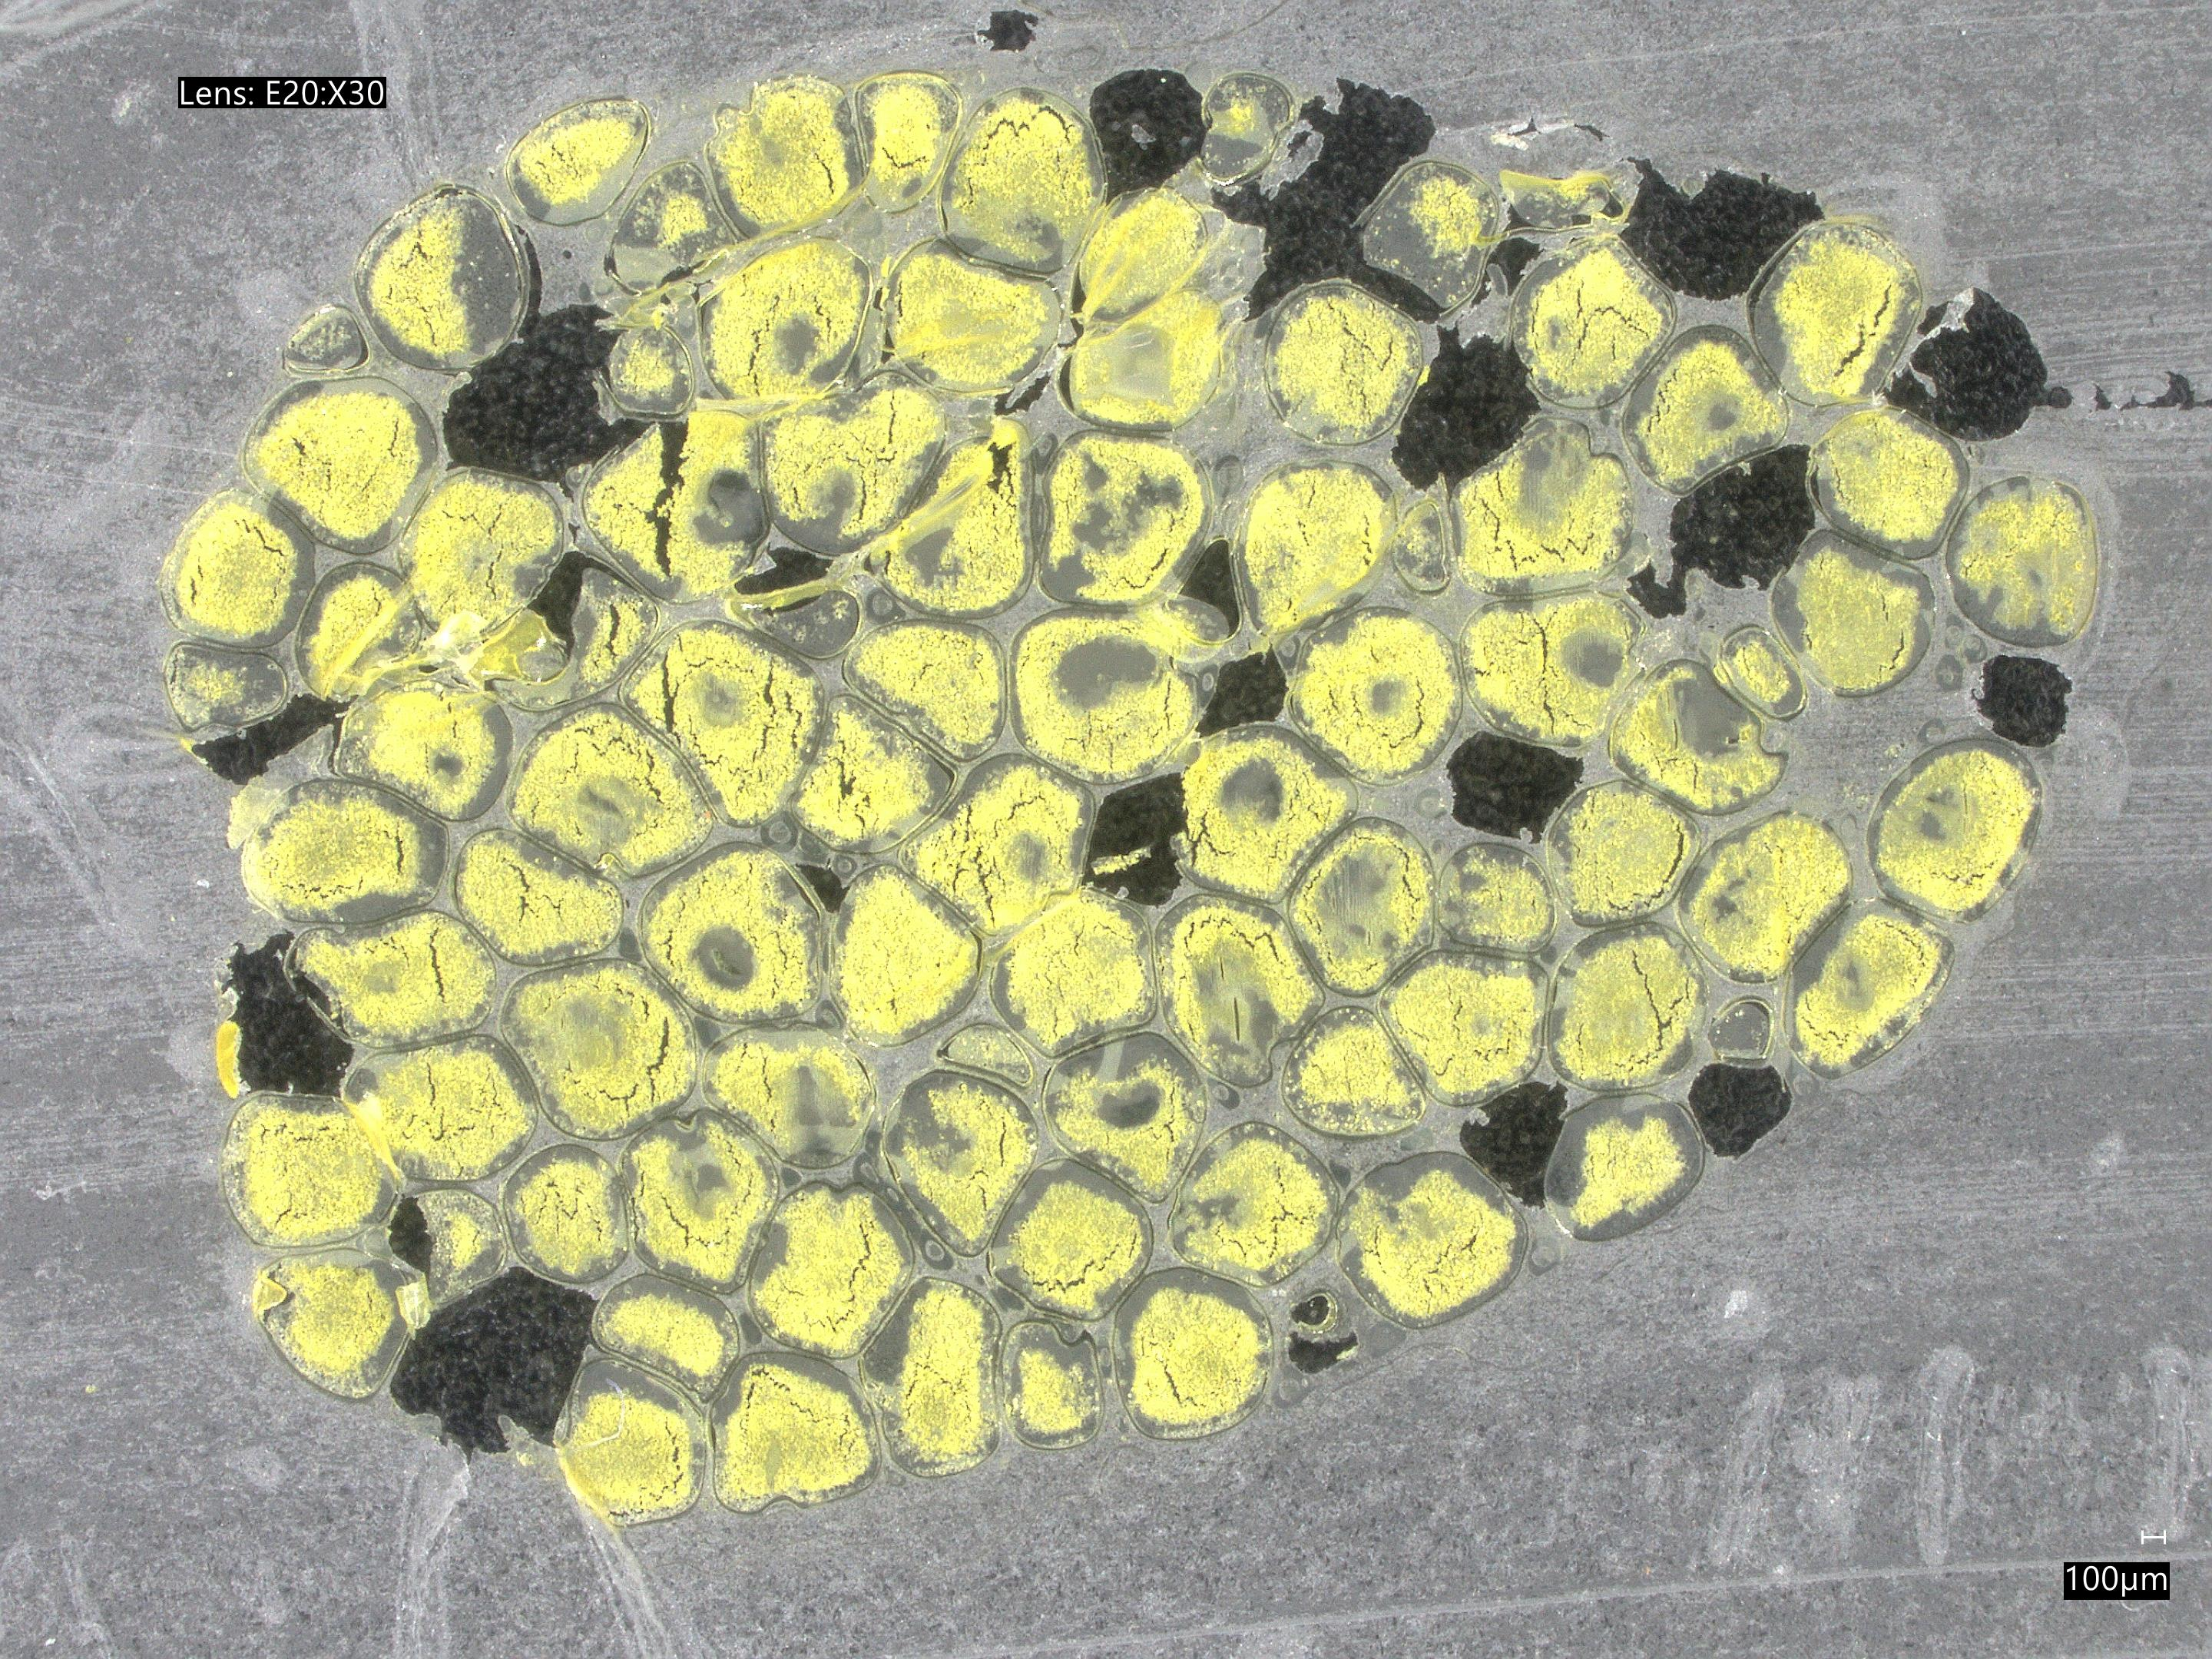
\includegraphics[width=\textwidth]{./fig/fish_lung/normal20240313_141726.jpg}
        \caption{normal fish lung}
        \label{fig:noraml_fish_lung}
    \end{minipage}
\end{figure}

\begin{figure}[H]
    \centering
    \begin{minipage}{0.45\textwidth}
        \centering
        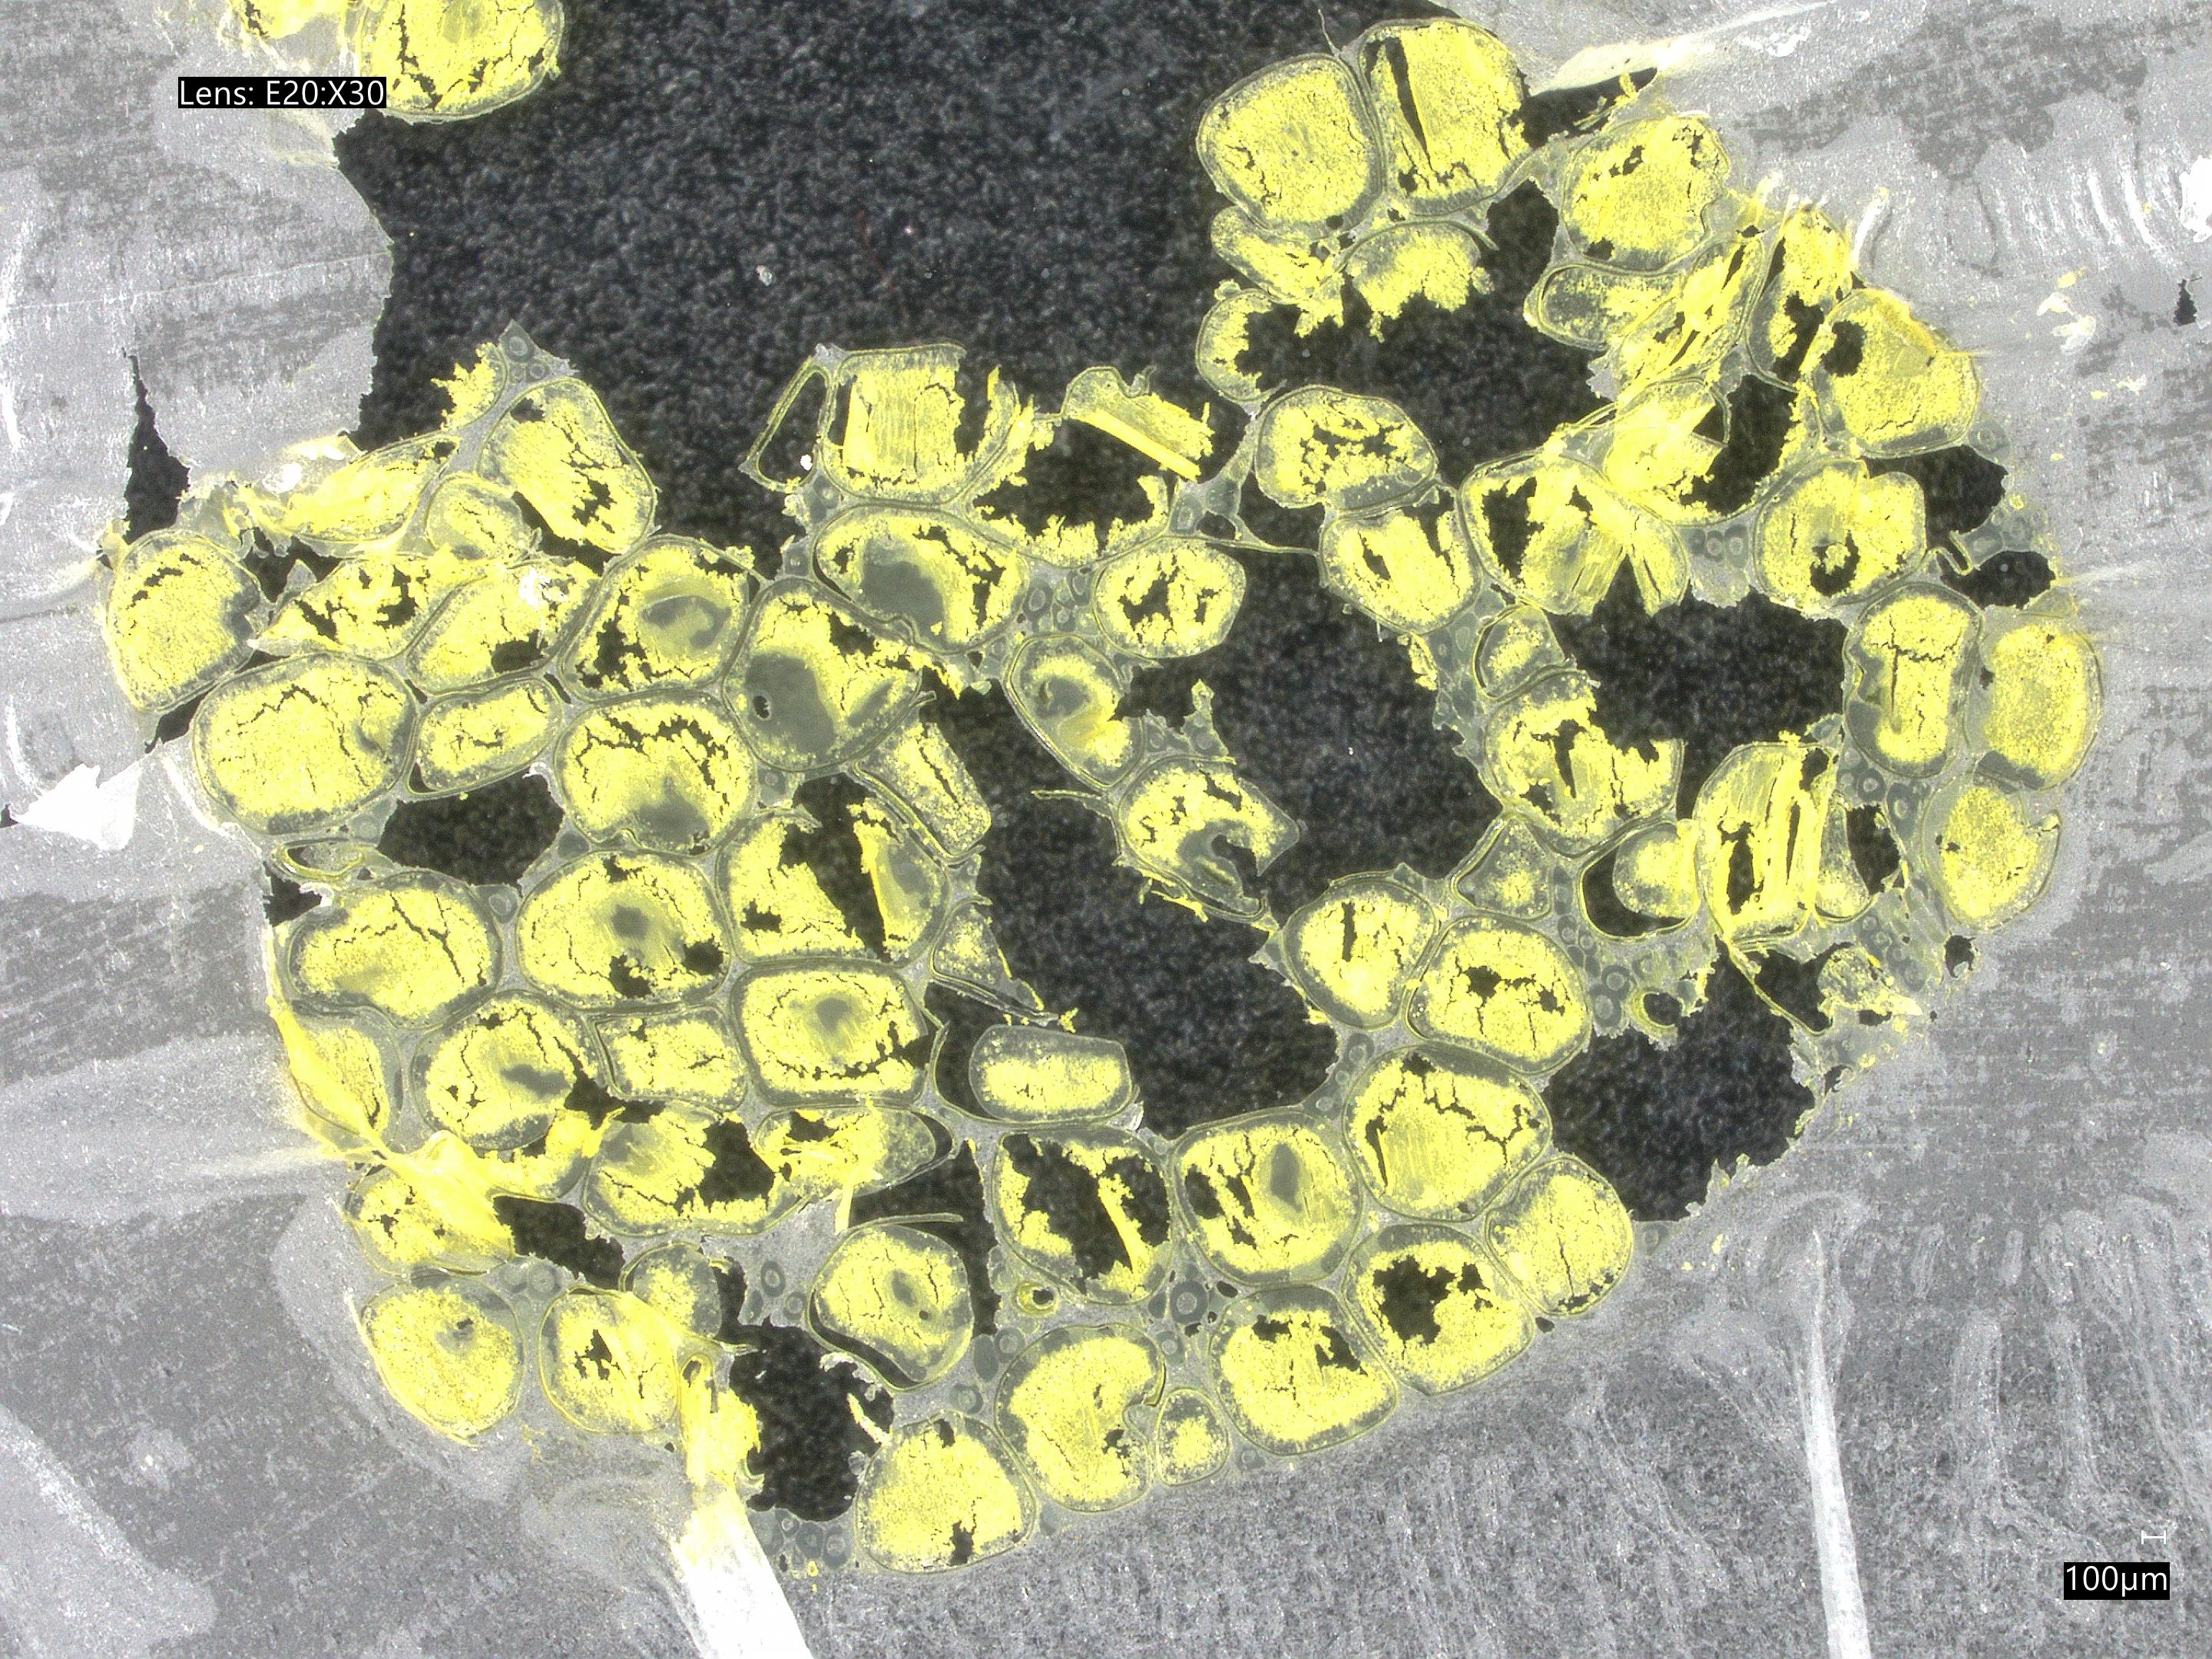
\includegraphics[width=\textwidth]{./fig/fish_lung/bad20240313_140952.jpg}
        \caption{bad fish lung}
        \label{fig:bad_fish_lung}
    \end{minipage}
    \begin{minipage}{0.45\textwidth}
        \centering
        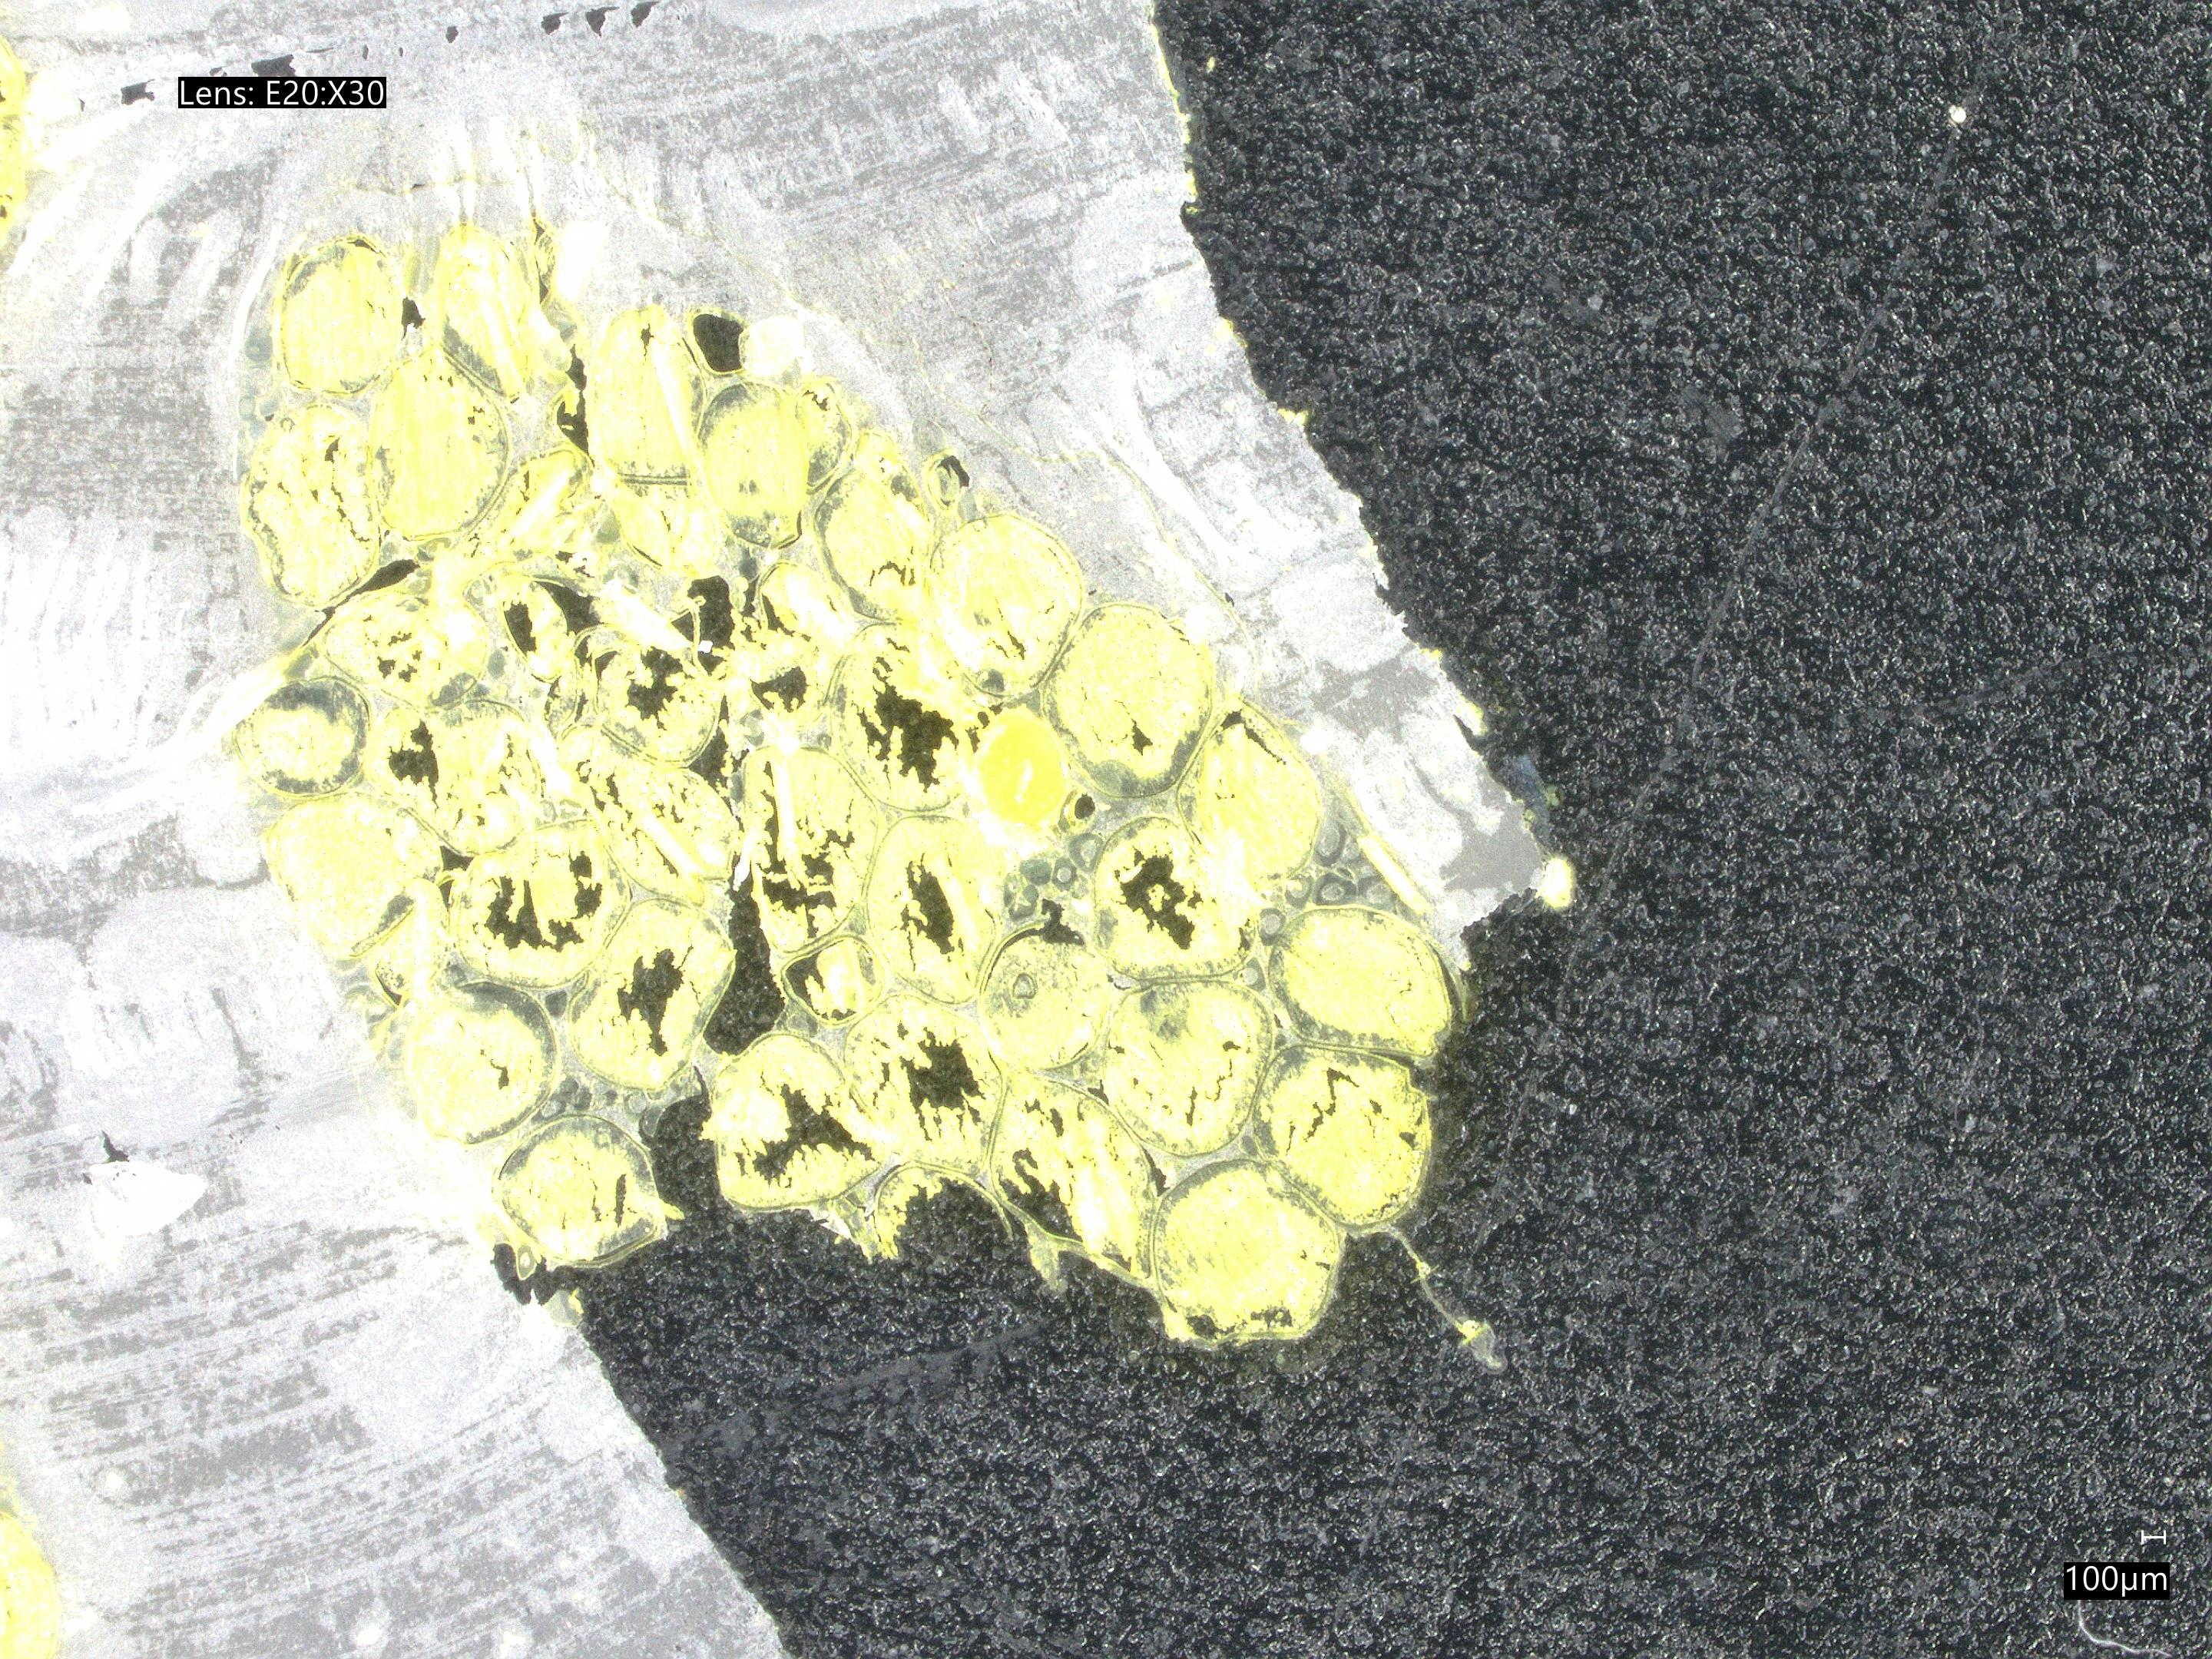
\includegraphics[width=\textwidth]{./fig/fish_lung/other20240313_141858.jpg}
        \caption{other fish lung}
        \label{fig:other_fish_lung}
\end{minipage}
\end{figure}


训练的准确度和损失如\autoref{fig:model5_acc}和\autoref{fig:model5_loss}所示。
\begin{figure}[H]
    \centering
    \begin{minipage}{0.45\textwidth}
        \centering
        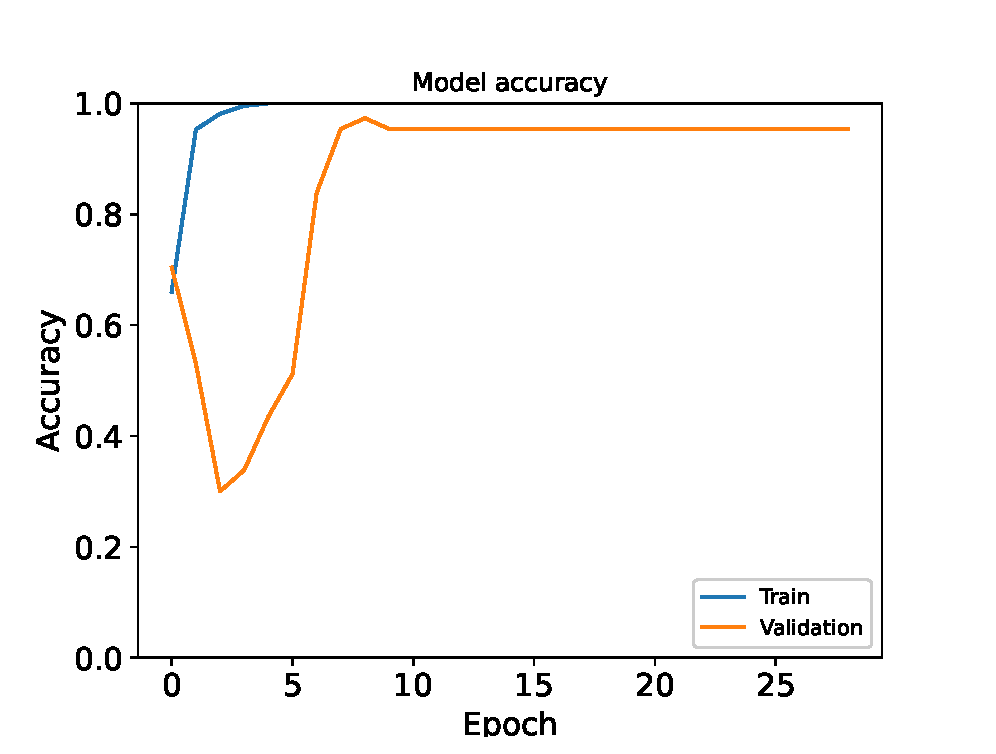
\includegraphics[width=\textwidth]{./fig/fish_lung/accuracy5.eps}
        \caption{Model-5 accuracy}
        \label{fig:model5_acc}
    \end{minipage}
    \begin{minipage}{0.45\textwidth}
        \centering
        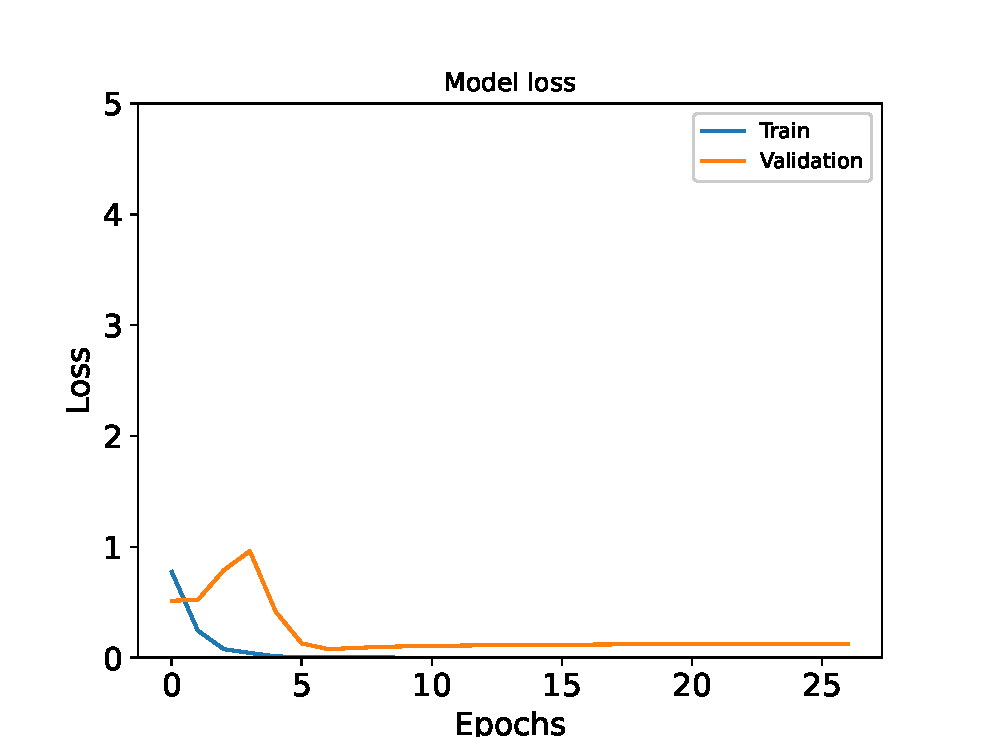
\includegraphics[width=\textwidth]{./fig/fish_lung/loss5.eps}
        \caption{Model-5 loss}
        \label{fig:model5_loss}
    \end{minipage}
\end{figure}

通过观察图片可以得出:
模型5的训练和验证准确度迅速上升并保持在高位,表明模型在这两个数据集上均有良好表现,损失图显示训练损失快速降低并趋于零,而验证损失在初始阶段出现尖峰后迅速降低并稳定,整体来看,这些迹象表明模型具有较好的拟合能力和泛化性能。

将其带入测试集进行测试,结果如\autoref{fig:accuracy_histogram2}所示:

\begin{figure}[H]
    \begin{minipage}{0.45\textwidth}
        \centering
        \captionof{table}{Model accuracy on test set}
        \begin{tabular}{ccccc}
            \toprule
            label & accuracy(\%) \\
            \midrule
            bad & 94.1 \\
            good & 98.2 \\
            normal & 94.7 \\
            other & 95.0 \\
            \bottomrule
        \end{tabular}
        \label{tab:model_accuracy3}
    \end{minipage}
    \begin{minipage}{0.45\textwidth}
        \centering
        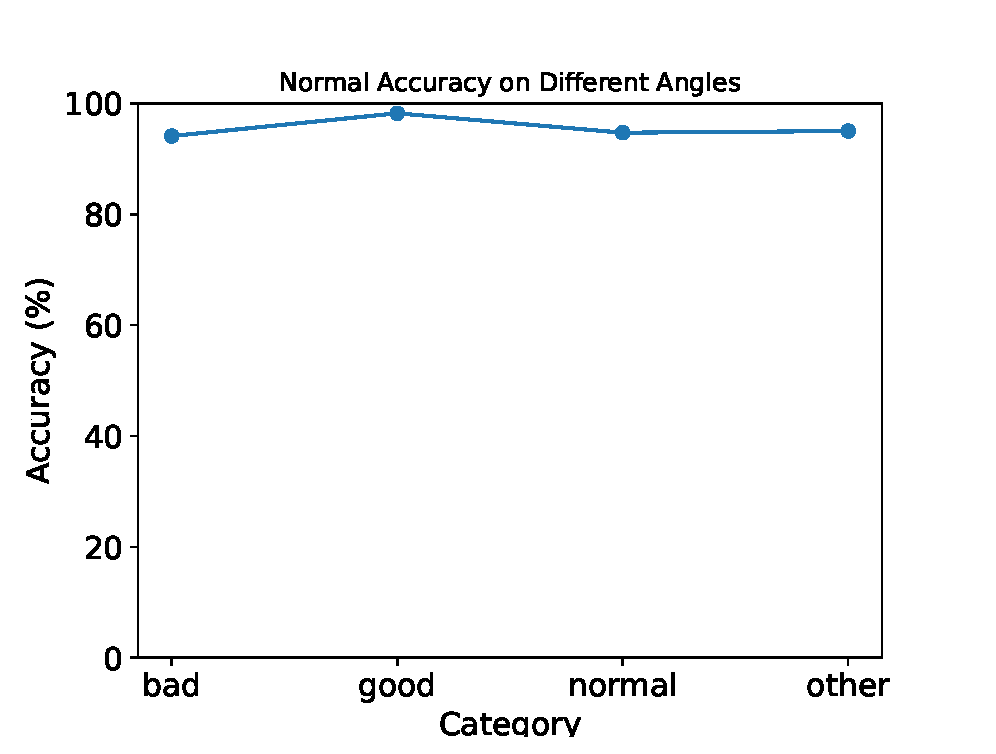
\includegraphics[width=\textwidth]{./fig/assistplot/angle_accuracy2.eps}
        \caption{Model Accuracy on Test Set}
        \label{fig:accuracy_histogram2}
    \end{minipage}
\end{figure}

可见,模型预测结果在全部的标签中均有90\%以上的准确度,表现非常理想。这说明模型具有较好的通用性,可以应用到其他组织切片的分类中。

% (补充额外的表格-关于遇到肺泡验证准确度的表格)



\FloatBarrier